\documentclass[12pt,a4paper]{report}
\usepackage[utf8]{inputenc}
\usepackage{titlepic}
\usepackage{pdfpages}
\usepackage{graphicx}




\begin{document}
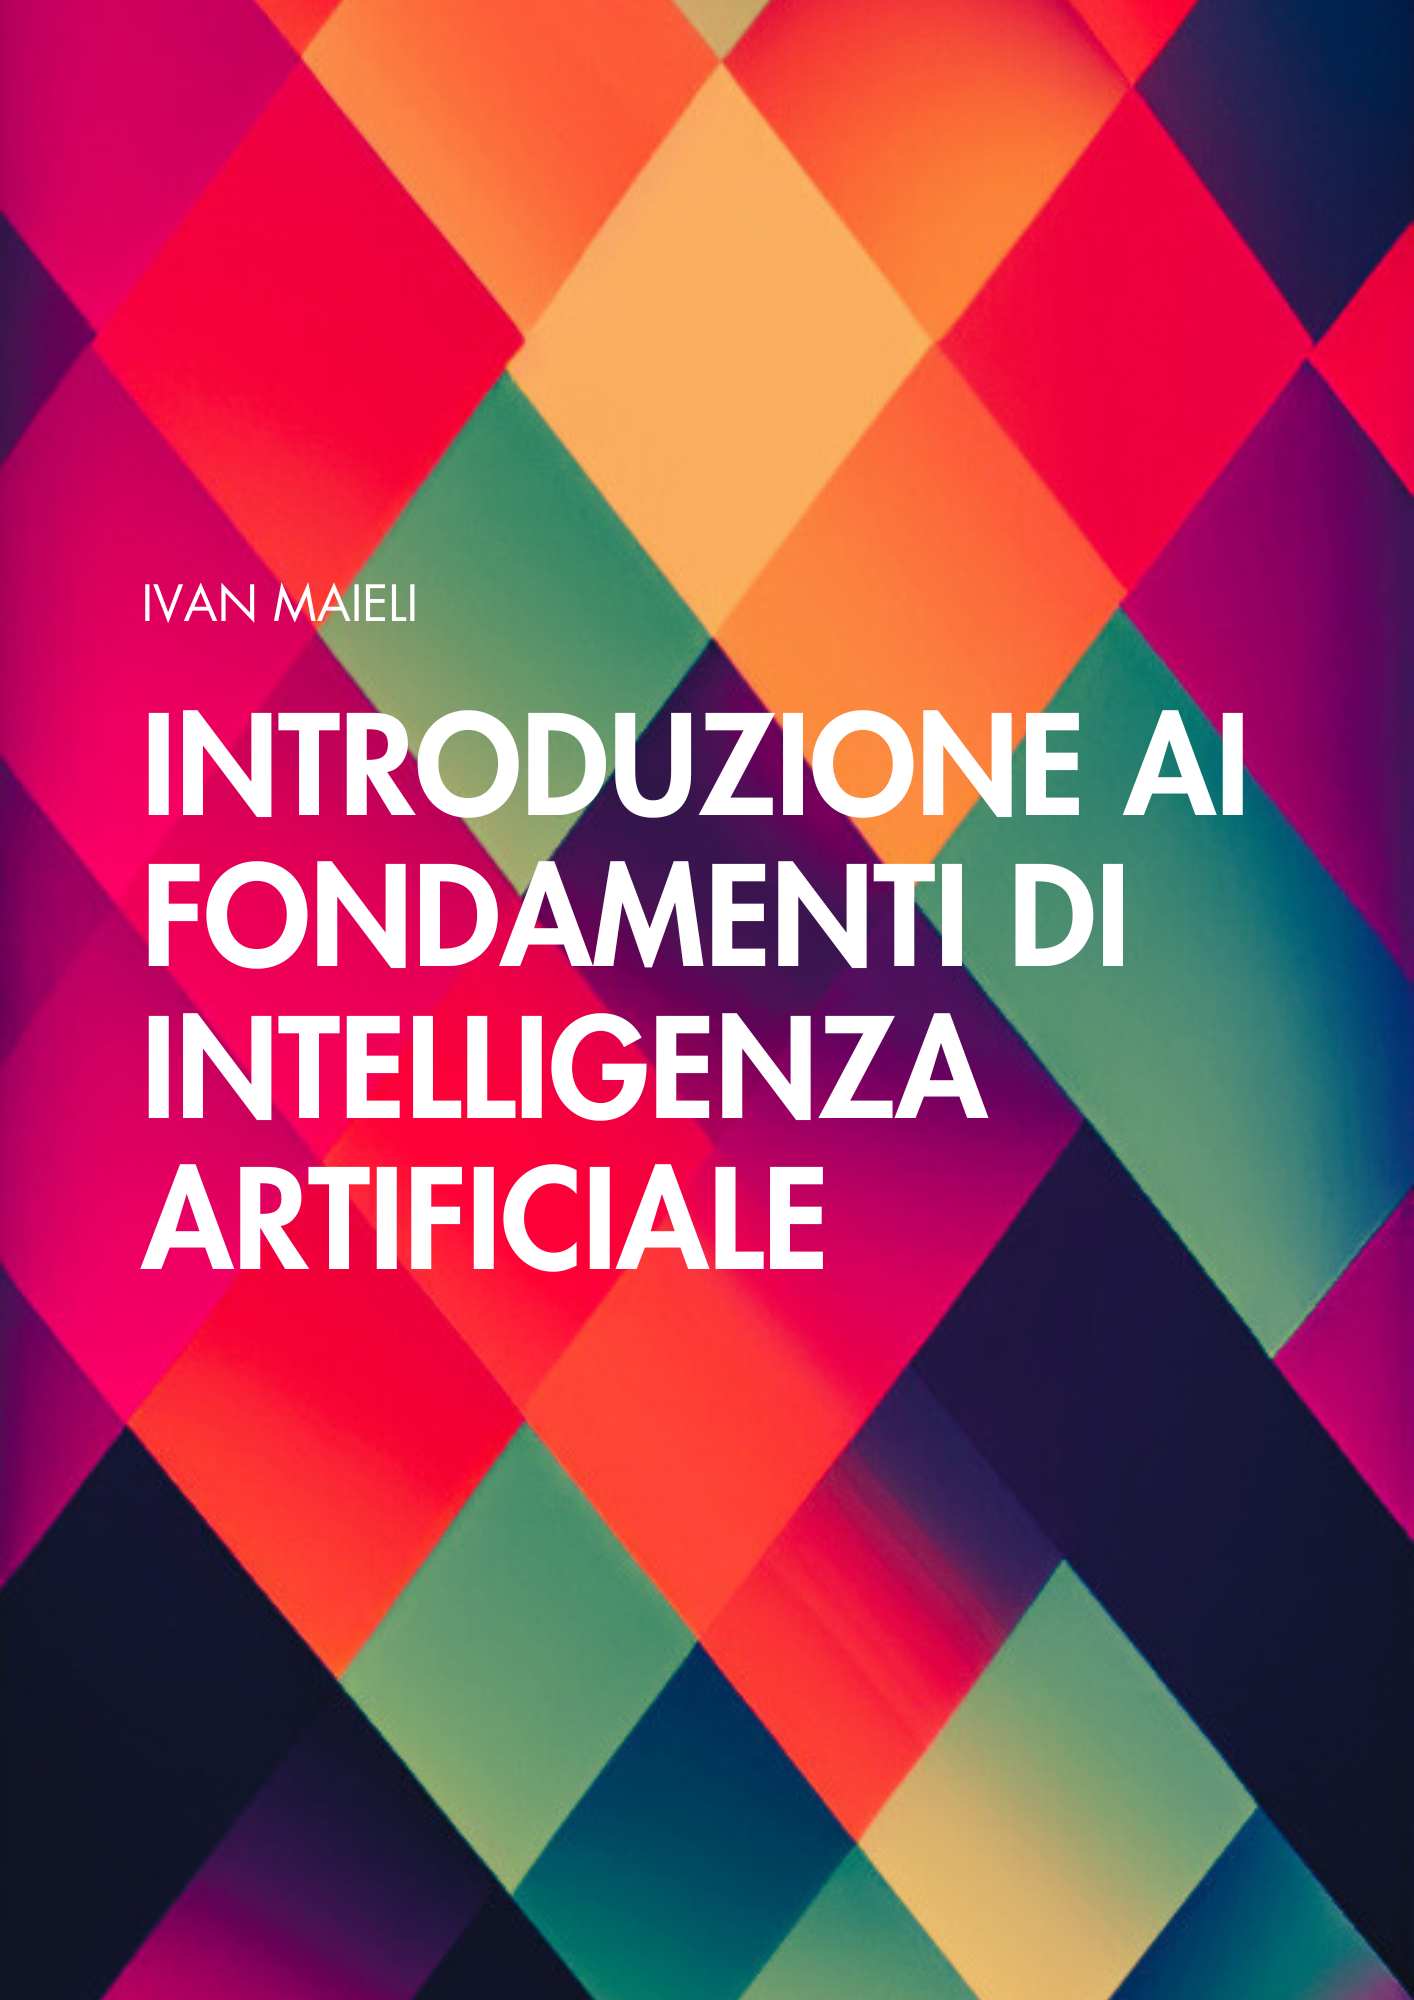
\includepdf[pages=1]{Covers/cover2.png}


\newpage

\tableofcontents

\newpage

\section*{Prefazione}
\textit{
Saluti a tutti i lettori interessati. \\
Il presente documento è redatto al fine di presentare un'offerta di supporto specializzato per il workshop sull'intelligenza artificiale assegnatoci dai rappresentanti della scuola "E. Fermi" di Siracusa. \\
Il laboratorio si concentra su argomenti di base relativi all'intelligenza artificiale, proponendo un breve corso di durata approssimativa di due ore. \\
Durante questo intervallo temporale, sarà esaminato un algoritmo specifico, ritenuto ottimale per una prima introduzione all'argomento.\\
Con l'obiettivo di fornire una panoramica storica e teorica esaustiva, è stata inclusa un'ampia gamma di informazioni, comprese nozioni di cultura generale, miti legati alle intelligenze artificiali e le corrispondenti verità. \\
Questa scelta metodologica mira a fornire un quadro completo dell'evoluzione storica e del contesto teorico in cui si sviluppa l'intelligenza artificiale.\\
La partecipazione a questo workshop non richiede competenze specializzate, ma solo una comprensione di base di algebra, la familiarità con il concetto di funzione in ambito matematico e una cognizione essenziale sul funzionamento di uno script generico. \\
Questa scelta mira a rendere il contenuto accessibile a un pubblico eterogeneo, garantendo un'esperienza formativa inclusiva. \\
Il documento nasce dalla necessità di diffondere informazioni accurate sull'intelligenza artificiale, campo spesso soggetto a disinformazione e interpretazioni errate. \\
L'obiettivo è quello di fornire una base informativa solida, contrastando voci di corridoio e congetture fantascientifiche che possono influenzare erroneamente la percezione dell'intelligenza artificiale. \\
Mi auguro che i contenuti presentati in questo workshop siano di valore e di gradimento per gli interessati. 
\begin{flushright}
Ivan Maieli
\end{flushright}
}
\newpage
\chapter{Introduzione ai Fondamenti di Intelligenza Artificiale}
\section{Definizione di Intelligenza Artificiale}
\textit{L'Intelligenza Artificiale (IA) è un campo di studio che si occupa di sviluppare sistemi e programmi in grado di eseguire compiti che richiedono intelligenza umana. L'obiettivo principale dell'IA è quello di creare macchine capaci di apprendere, ragionare e prendere decisioni in modo autonomo.\\
\\
} 
Questa rappresenta la comune definizione adottata e riconosciuta che, solitamente, rappresenta anche un approccio sorprendentemente concreto ad un campo così attratto.  
Vi avviso: tra poche righe vedrete tante altre definizioni, perlopiù "rubate" (preferirei dire "prese in prestito") da fonti valide, come personaggi illustri o aziende. \\
In questa sezione preferisco di gran lunga inserire molteplici definizioni, poiché non esiste quasi mai una verità assoluta quando parliamo di Intelligenze Artificiali e, proprio per questo motivo, apprezzerei un vostro sforzo nell'orientarci verso una strada critica, e non comune.\\ \\
Ecco cosa ci dicono i fondatori della materia: \\ \\
\textit{L'obiettivo finale dell'intelligenza artificiale è costruire agenti che sono in grado di superare gli esseri umani in quasi tutti i compiti di interesse generale.}
\begin{flushright}
Demis Hassabis, cofondatore di DeepMind
\end{flushright}
\textit{\\L'intelligenza artificiale è la scienza e l'ingegneria di fare macchine intelligenti, in particolare programmando computer per eseguire funzioni cognitive.}
\begin{flushright}
John McCarthy, uno dei padri fondatori dell'intelligenza artificiale
\end{flushright}
\textit{\\L'IA è lo studio di come far svolgere alle macchine cose che altrimenti richiederebbero l'intelligenza umana.}
\begin{flushright}
Marvin Minsky, cofondatore del MIT Artificial Intelligence Project 
\end{flushright}
\textit{\\L'intelligenza artificiale sarà più di una semplice collezione di strumenti e tecnologie, sarà il più grande evento nella storia umana.}
\begin{flushright}
Ray Kurzweil, Direttore dell'Ingegneria presso Google
\end{flushright}
\textit{\\Qualsiasi cosa che un essere umano possa fare con meno di un secondo di riflessione, possiamo ora automatizzarla utilizzando l'IA.}
\begin{flushright}
Andrew Ng, co-fondatore di Google Brain
\end{flushright}

Le definizioni di intelligenza artificiale (IA) nel corso del tempo spaziano da concetti più specifici e orientati alle capacità di apprendimento automatico e ragionamento delle macchine, a prospettive più ampie che includono la simulazione di comportamenti intelligenti. \\
Il punto d'incontro tra queste definizioni spesso riguarda la capacità delle macchine di emulare alcune funzioni cognitive umane. \\
Possiamo notare come in molte di esse sia presente la chiave \textit{rapidità}, che contraddistingue le scelte compiute dalle IA, basate su calcoli e probabilità, e non su sensi di colpa e pregiudizi (a meno che non addestriamo la nostra IA proprio per questi scopi, ma noi non vogliamo). \\
Ricordiamo sempre che tecnologie di questo tipo debbano sempre e comunque essere utilizzate per scopi che \textbf{migliorino} la vita dell'umanità, nei confronti della quale dovrebbe servirsi l'ingegneria.
\\
\\
\\
\\
\section{Storia dell'Intelligenza Artificiale}
La storia delle intelligenze artificiali ha una fase chiave legata allo sviluppo del perceptron, un concetto fondamentale nel campo delle reti neurali. Il perceptron rappresenta un punto di svolta nei primi anni '60 e ha contribuito a plasmare la direzione dell'intelligenza artificiale (IA) in quel periodo. \\
è stato proposto da Frank Rosenblatt nel 1957 come un modello semplificato di neurone biologico. Questo modello ha introdotto l'idea che una macchina potrebbe apprendere attraverso l'adattamento dei pesi associati agli input, ispirandosi alla maniera in cui i neuroni del cervello umano sembrano funzionare. \\
Nel 1958, Rosenblatt costruì il primo dispositivo fisico basato sul perceptron chiamato "Mark I Perceptron". Questa macchina aveva la capacità di apprendere dai dati attraverso un processo di adattamento dei pesi delle connessioni tra i neuroni artificiali, permettendogli di riconoscere pattern e compiere semplici decisioni.
Tuttavia, aveva limitazioni. \\
Una delle critiche principali proveniva da Marvin Minsky e Seymour Papert nel loro libro del 1969, "Perceptrons," dove dimostrarono che un singolo perceptron non era in grado di risolvere problemi complessi come la XOR (esclusiva logica o). \\
Questa limitazione portò a una diminuzione dell'interesse nell'utilizzo di perceptron e reti neurali in generale, contribuendo al periodo noto come "inverno dell'IA."\\
Nonostante ciò, la concezione del perceptron e il concetto di apprendimento tramite l'adattamento dei pesi hanno fornito le fondamenta per lo sviluppo futuro delle reti neurali. \\
Gli anni '80 e '90 hanno visto una rinascita dell'interesse nell'apprendimento automatico e nelle reti neurali grazie a nuove tecniche e algoritmi, come le reti neurali profonde.\\
Oggi, il perceptron è considerato una pietra miliare nella storia delle IA, nonostante le sue limitazioni iniziali.\\ La sua evoluzione ha contribuito a plasmare la direzione dell'apprendimento automatico e delle reti neurali, che sono diventate elementi chiave nell'odierna avanzata intelligenza artificiale.\\
La storia moderna delle intelligenze artificiali è caratterizzata da una notevole accelerazione degli sviluppi e da una diffusione su vasta scala in diversi settori. \\
Negli ultimi decenni, molteplici fattori, come l'aumento della potenza di calcolo, la disponibilità di enormi quantità di dati e i progressi negli algoritmi, hanno contribuito a trasformare radicalmente il panorama dell'IA. \\
Negli anni '90 e nei primi anni 2000, l'IA ha iniziato a essere sempre più integrata nella vita quotidiana. Sono emersi sistemi di raccomandazione, motori di ricerca avanzati e assistenti vocali. \\
Il riconoscimento del linguaggio naturale e la comprensione delle immagini hanno registrato progressi significativi, portando a miglioramenti nei servizi online e nella gestione delle informazioni. \\
Il periodo più recente ha visto l'ascesa dell'apprendimento profondo e delle reti neurali profonde. Queste architetture neurali, ispirate vagamente al funzionamento del cervello umano, hanno dimostrato straordinarie capacità nel campo della visione artificiale, del riconoscimento del linguaggio naturale e in molti altri compiti. \\
Le reti neurali profonde sono alla base di molte applicazioni di successo, come il riconoscimento facciale, la guida autonoma, e la traduzione automatica.
Settori come la salute, la finanza, la logistica e la produzione hanno beneficiato dell'implementazione dell'IA per ottimizzare processi, prendere decisioni più informate e sviluppare soluzioni più efficienti. \\
L'IA è anche diventata uno strumento prezioso nella ricerca scientifica, facilitando l'analisi dei dati e la scoperta di modelli incomprensibili per l'occhio umano.
Parallelamente, l'etica e la responsabilità nell'uso dell'Intelligenza Artificiale sono diventate preoccupazioni cruciali.\\ L'espansione dell'IA ha sollevato questioni relative alla sicurezza, alla privacy e alla potenziale perdita di posti di lavoro. \\
Ci sono crescenti sforzi per sviluppare normative e linee guida che regolamentino l'uso dell'IA e ne assicurino un'applicazione etica.\\
\\
\\
\section{Amo i film di fantascienza, davvero}
I film di fantascienza spesso ritraggono intelligenze artificiali come entità distruttive o come minacce per l'umanità. Questi racconti sono spesso basati su elementi drammatici e narrativi, ma è importante sottolineare che essi rappresentano scenari estremi e poco realistici rispetto allo stato attuale dell'IA e alla sua evoluzione futura. \\
\\
Mito: Le IA saranno necessariamente ostili all'umanità.\\
Realtà: L'IA è uno strumento sviluppato e utilizzato dagli esseri umani. La sua natura dipenderà dagli scopi per cui è stata progettata. Molti ricercatori e sviluppatori si concentrano sulla creazione di IA etiche e sicure.\\
\\
Mito: Le IA saranno sempre più intelligenti degli esseri umani e si ribelleranno.\\
Realtà: Non esiste un consenso sulla possibilità di raggiungere un livello di intelligenza sovrumana nelle IA. Inoltre, gli sviluppatori spesso integrano limiti di sicurezza per evitare scenari catastrofici. \\
\\
Mito: Le IA svilupperanno una volontà propria indipendente dagli obiettivi umani.\\
Realtà: L'IA è progettata per raggiungere obiettivi specifici stabiliti dagli sviluppatori. L'idea di una volontà indipendente è più fantascienza che realtà tecnologica.\\
\\
Mito: Gli esseri umani perderanno il controllo sulle IA.\\
Realtà: La sicurezza e il controllo sono aspetti fondamentali nello sviluppo delle IA. Gli esperti stanno lavorando per implementare misure che permettano di mantenere il controllo e prevenire usi indesiderati.\\
\\
Mito: Tutte le IA saranno simili a Skynet di "Terminator" o HAL di "2001: Odissea nello spazio".\\
Realtà: Le rappresentazioni di IA come Skynet e HAL sono drammatizzate per fini narrativi. La maggior parte delle IA reali è specializzata in compiti specifici e non ha la complessità o l'ambizione di queste rappresentazioni cinematografiche.\\
\\
Mito: Le IA non possono essere controllate. \\
Realtà: Gli sforzi per sviluppare IA responsabili includono normative, etica nella progettazione e sviluppo di meccanismi di controllo e sicurezza.\\
\chapter{Un computer è molto più stupido di quanto pensiate}
\section{I dati sono davvero importanti}
\section{Introduzione alla terminologia}
\section{Supervised Learning}
\section{Unsupervised Learning}
\section{Reinforcement Learning}

\chapter{Gallina vecchia fa buon brodo: il Perceptron}
\section{Non è magia}
\section{La matematica}
\subsection{Gestione degli Input}
\subsection{Funzioni di attivazione}
\subsection{Calcolo errore}
\subsection{Aggiornamento pesi}
\section{I limiti}

\chapter{Il nostro primo (e unico) progetto}
\section{Descrizione}
\section{Finalmente un po' di codice}


\end{document}


